% Build from this directory with: latexmk -pdf main.tex
% A single pdflatex pass does not resolve the bibliography or cross-references.
\documentclass[11pt]{article}

% Change "review" to "final" to generate the final (sometimes called camera-ready) version.
% Change to "preprint" to generate a non-anonymous version with page numbers.
\usepackage[]{acl}
\usepackage{times}
\usepackage{latexsym}

% For proper rendering and hyphenation of words containing Latin characters (including in bib files)
\usepackage[T1]{fontenc}
% For Vietnamese characters
% \usepackage[T5]{fontenc}
% See https://www.latex-project.org/help/documentation/encguide.pdf for other character sets

% This assumes your files are encoded as UTF8
\usepackage[utf8]{inputenc}
\usepackage{microtype}
\usepackage{inconsolata}
\usepackage{graphicx}
\usepackage{array}
\usepackage{amsmath}

% If the title and author information does not fit in the area allocated, uncomment the following
%
%\setlength\titlebox{<dim>}
%
% and set <dim> to something 5cm or larger.

\title{Group 32 Progress Report:\\Predicting Purchase Outcomes from Online Shopping Session Behavior}


\author{Ankur Pandey, Allen Tong, Krish Haryani \\
  \texttt{\{pandea23,tonga17,haryanik\}@mcmaster.ca} }

%\author{
%  \textbf{First Author\textsuperscript{1}},
%  \textbf{Second Author\textsuperscript{1,2}},
%  \textbf{Third T. Author\textsuperscript{1}},
%  \textbf{Fourth Author\textsuperscript{1}},
%\\
%  \textbf{Fifth Author\textsuperscript{1,2}},
%  \textbf{Sixth Author\textsuperscript{1}},
%  \textbf{Seventh Author\textsuperscript{1}},
%  \textbf{Eighth Author \textsuperscript{1,2,3,4}},
%\\
%  \textbf{Ninth Author\textsuperscript{1}},
%  \textbf{Tenth Author\textsuperscript{1}},
%  \textbf{Eleventh E. Author\textsuperscript{1,2,3,4,5}},
%  \textbf{Twelfth Author\textsuperscript{1}},
%\\
%  \textbf{Thirteenth Author\textsuperscript{3}},
%  \textbf{Fourteenth F. Author\textsuperscript{2,4}},
%  \textbf{Fifteenth Author\textsuperscript{1}},
%  \textbf{Sixteenth Author\textsuperscript{1}},
%\\
%  \textbf{Seventeenth S. Author\textsuperscript{4,5}},
%  \textbf{Eighteenth Author\textsuperscript{3,4}},
%  \textbf{Nineteenth N. Author\textsuperscript{2,5}},
%  \textbf{Twentieth Author\textsuperscript{1}}
%\\
%\\
%  \textsuperscript{1}Affiliation 1,
%  \textsuperscript{2}Affiliation 2,
%  \textsuperscript{3}Affiliation 3,
%  \textsuperscript{4}Affiliation 4,
%  \textsuperscript{5}Affiliation 5
%\\
%  \small{
%    \textbf{Correspondence:} \href{mailto:email@domain}{email@domain}
%  }
%}

\begin{document}
\maketitle
% \begin{abstract}
% \end{abstract}

\section{Introduction}

Most visits to an online store end without a purchase. If a retailer could
estimate, from the way a session unfolds, how likely it is to end in a
purchase, it could learn which browsing patterns are associated with
conversion and where its website could be improved. Our project builds a
machine learning application that makes this estimate for individual
e-commerce sessions.

We frame the task as supervised, single-label binary classification on
tabular data. Each record in the UCI Online Shoppers Purchasing Intention
Dataset \citep{sakar2018dataset} summarizes one session with 17 inputs: page
counts and time spent on administrative, informational and product pages;
bounce and exit rates; the PageValues analytics measure; calendar context; and
device, region, traffic-source and visitor-type categories. The target,
\texttt{Revenue}, records whether the session ended in a purchase. The model
estimates a purchase probability and assigns a class using a probability
threshold selected on validation data.

Three properties make the problem harder than it first appears. First,
purchases are rare: only 15.5\% of the 12,330 sessions end in a purchase, so a
model that always predicts ``no purchase'' is 84.5\% accurate while being
useless. Second, shopper behavior is heterogeneous, and the activity measures
are long-tailed. Third, a single analytics feature, PageValues, carries much
of the signal. In our training split, 55.6\% of sessions with a positive
PageValues end in a purchase, compared with 3.9\% of sessions where it is zero.
However, PageValues is derived from the value of pages that previously led to
transactions. Not every website records it, sites may compute it differently,
and it is unclear whether it would be available before a purchase is made. A
model that relies on it may therefore be less reliable outside this dataset.

Our contribution is not a new leaderboard result on this dataset. Instead, we
aim to provide (i) a careful comparison of majority-class baselines,
regularized logistic regression, random forest and XGBoost under a fixed,
leakage-aware evaluation protocol; (ii) a feature-availability study that
compares all 17 inputs with subsets that exclude PageValues and, optionally,
the bounce and exit rates; (iii) calibrated purchase probabilities rather than
labels alone; and (iv) an inspectable Streamlit demonstration that returns
probabilities, predicted classes and influential inputs for a session summary.
Our results describe session-summary classification on one website and do not
establish generalization to future periods or other stores.

\section{Related Work}

\paragraph{Purchase intent on this dataset.}
The dataset was introduced by \citet{sakar2019realtime}, who proposed a
real-time system with two modules. The first module predicts purchasing
intention from session-level aggregate features like ours, comparing a
multilayer perceptron with other classifiers such as random forests and
support vector machines, and using oversampling and feature selection to
address class imbalance. The second module uses an LSTM recurrent network on
sequential clickstream data to estimate the likelihood that a visitor will
leave the site. Our work extends their session-level study in two directions:
we explicitly measure how much performance depends on PageValues and other
analytics-derived inputs, and we evaluate probability quality in addition to
classification accuracy.

\paragraph{Clickstream models of conversion.}
Earlier marketing research modeled conversion directly from browsing
behavior. \citet{moe2004dynamic} modeled each visitor's probability of
buying as it evolves across repeated visits, accounting for differences
between shoppers, and showed that conversion behavior changes over time.
\citet{montgomery2004clickstream} modeled the sequence of pages a user views
and showed that the browsing path carries information that improves
predictions of purchase conversion. Our dataset contains only per-session
summaries without raw page sequences, so we cannot use path models directly,
but these studies motivate the page-count and duration inputs we use.

\paragraph{Models for tabular data.}
Our candidate models are standard strong performers on structured data.
Random forests \citep{breiman2001random} average many decorrelated decision
trees, and XGBoost \citep{chen2016xgboost} is a regularized,
scalable implementation of gradient-boosted trees. A comparison by
\citet{shwartzziv2022tabular} found that XGBoost generally matched or
outperformed recent deep learning models on tabular benchmarks while
requiring less tuning, which supports our choice to focus on tree ensembles and a
logistic regression baseline instead of a neural network.

\paragraph{Imbalance, evaluation and calibration.}
\citet{he2009imbalanced} survey learning from imbalanced data, including
resampling and cost-sensitive methods, and note that overall accuracy can
be misleading when one class dominates. Following \citet{saito2015precision},
who show that precision--recall analysis is more informative than ROC
analysis when positives are rare, we use purchase-class average precision as
our primary metric. \citet{niculescu2005predicting} show that common learners
such as boosted trees and random forests can produce systematically distorted
probabilities that calibration methods correct, which motivates our use of
Brier scores and reliability plots. Finally, \citet{kaufman2012leakage}
describe how features that would not be available at prediction time can
inflate reported performance. This concern underlies our PageValues study
and our decision to fit all preprocessing within training folds only.

\section{Dataset}

\subsection{Source and structure}

We use the complete UCI Online Shoppers Purchasing Intention Dataset
\citep{sakar2018dataset}, introduced by \citet{sakar2019realtime} and
distributed as a single CSV file under a CC BY 4.0 license. It contains
12,330 sessions, each from a different user over a one-year period, with 17
input features and the Boolean target \texttt{Revenue}, which records whether
the session ended in a purchase (not the amount spent). No scraping, API
access or manual annotation was required, since every session already carries
its recorded outcome. Table~\ref{tab:features} summarizes the inputs.

\begin{table}[t]
  \centering
  \small
  \begin{tabular}{>{\raggedright\arraybackslash}p{0.52\columnwidth}>{\raggedright\arraybackslash}p{0.36\columnwidth}}
    \hline
    \textbf{Inputs} & \textbf{Type} \\
    \hline
    Administrative, Informational, ProductRelated (pages visited) & Count \\
    The three matching \texttt{\_Duration} fields (total time on each page type) & Continuous, units unspecified \\
    BounceRates, ExitRates & Fraction in $[0,1]$ \\
    PageValues (average value of pages visited before a transaction) & Continuous, currency unspecified \\
    SpecialDay (closeness to a holiday) & Score in $\{0, 0.2, \dots, 1\}$ \\
    Month, VisitorType & Nominal label \\
    OperatingSystems, Browser, Region, TrafficType & Nominal integer code \\
    Weekend & Boolean \\
    \hline
  \end{tabular}
  \caption{\label{tab:features}
    The 17 session-level inputs. Category codes have no documented meaning
    or order.}
\end{table}

\subsection{Properties of the data}

Before dividing the file, we audited it in its entirety. Every numeric field is non-negative, and there are no missing or blank values. Five characteristics of the data influenced our design.

\paragraph{Class imbalance.} Only 1,908 sessions (15.5\%) end in a purchase,
against 10,422 non-purchases. A classifier that never predicts a purchase is
84.5\% accurate, which is why we do not use accuracy as our main metric
(Section~\ref{sec:results}).

\paragraph{Skewed activity and meaningful zeros.} All ten numeric inputs are
positively skewed. Product-page time has a median of 598.9 but a maximum of
63,974, and sessions view a median of 18 product pages but only one
administrative page and no informational pages. Zeros are common and
informative rather than missing: PageValues is zero for 77.9\% of sessions,
and SpecialDay for 89.9\%. Bounce and exit rates both stop at 0.2, with about
700 sessions each at exactly that value, which suggests a boundary in how the
source computed them.

\paragraph{Correlated inputs.} On the training split, each page count is
strongly rank-correlated with its duration (Spearman $\rho$ of 0.88--0.95),
and bounce and exit rates are moderately correlated ($\rho = 0.60$).
PageValues has by far the strongest association with purchase
($\rho = 0.62$), as discussed in the introduction.

\paragraph{Uneven categories.} January and April are absent entirely, and the
sessions per month range from 184 (February) to 3,364 (May). Purchase rates
also vary by group (Figure~\ref{fig:context}): 25.5\% of training sessions in
November end in a purchase compared with 2.1\% in February, and new visitors
purchase more often than returning visitors (23.9\% vs.\ 14.1\%). Several
browser, operating system and traffic-type codes occur fewer than 20 times,
and some occur only once.

\paragraph{Identical sessions.} 201 sessions fall into 76 groups whose 17
inputs are identical, and no group has conflicting labels. Because the data
has no user identifiers, we cannot tell whether these are true duplicates or
different users with the same summary, so we keep them all.

\begin{figure*}[t]
  \centering
  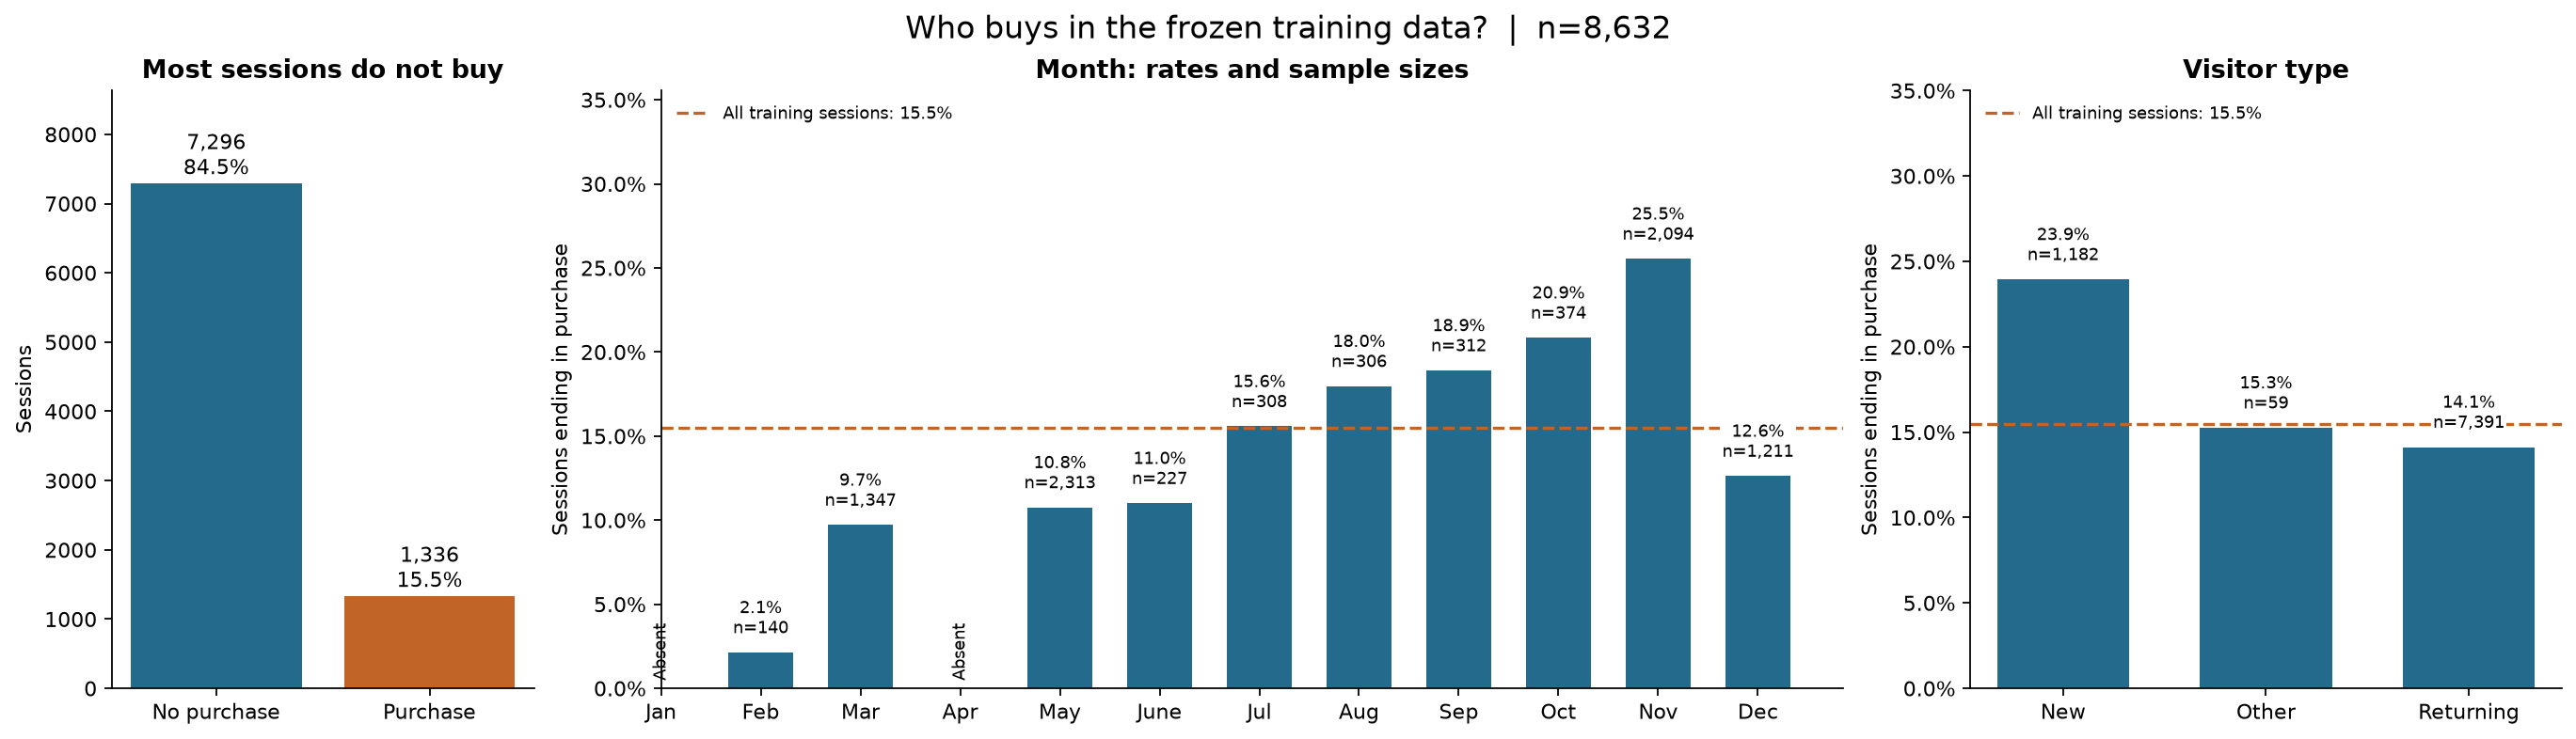
\includegraphics[width=\linewidth]{figures/purchase_context.png}
  \caption{\label{fig:context}
    Training split ($n = 8{,}632$). Left: class balance. Centre and right:
    share of sessions ending in a purchase by month and by visitor type, with
    sample sizes. The dashed line marks the overall purchase rate (15.5\%).}
\end{figure*}

\subsection{Preprocessing}
\label{sec:preprocessing}

We left the source file unchanged and removed no sessions, outliers or
repeated rows; extreme values are kept unless there is evidence they are
errors. All preprocessing decisions were made using the training split only.

\paragraph{Splitting.} We divided the sessions into training, validation and
test sets of 8,632, 1,849 and 1,849 sessions (about 70/15/15) with a fixed
random seed. The split is stratified, so each set keeps the 15.5\% purchase
rate, and grouped, so identical sessions always land in the same set. This
prevents a model from being evaluated on an exact copy of a training example.
The training set is further divided into five fixed cross-validation folds
under the same rules. The assignments are saved to files and verified on
every load, so every team member uses the same split
(Section~\ref{sec:results}).

\paragraph{Input checks and encoding.} Every session passes through an input
check that rejects missing values, negative counts, rates outside $[0, 1]$
and invalid category codes, without silently filling in or clipping values.
The six nominal fields are one-hot encoded, \texttt{Weekend} becomes a 0/1
indicator, and numeric inputs are standardized for logistic regression but
left unscaled for tree-based models. These steps are combined with each model
in a single scikit-learn pipeline, so the encoder's categories and the
scaler's statistics are learned from the training rows of each fold only.
Categories that were not seen during training are encoded as all zeros. With
all 17 inputs, this produces 74 model features (Section~\ref{sec:features}).

\paragraph{Limitations.} The released data contains session summaries only,
with no timestamps, year, user identifiers or page-by-page click sequences.
We therefore cannot build a time-ordered split or show that a model would
generalize to later periods or other websites.

\section{Features}
\label{sec:features}

Our models receive the 17 session-level inputs in Table~\ref{tab:features},
encoded as described in Section~\ref{sec:preprocessing}. Fitting the encoder
on the training split gives 74 model features (Table~\ref{tab:encoded}). Each
nominal field is represented by one indicator per observed level instead of
its integer code, since the codes have no documented order.

\begin{table}[t]
  \centering
  \small
  \begin{tabular}{lr}
    \hline
    \textbf{Input block} & \textbf{Columns} \\
    \hline
    Numeric inputs & 10 \\
    Month & 10 \\
    OperatingSystems & 8 \\
    Browser & 13 \\
    Region & 9 \\
    TrafficType & 20 \\
    VisitorType & 3 \\
    Weekend & 1 \\
    \hline
    \textbf{Total} & \textbf{74} \\
    \hline
  \end{tabular}
  \caption{\label{tab:encoded}
    Encoded model features for all 17 inputs, with category levels counted
    on the training split.}
\end{table}

\paragraph{Feature engineering.} We have not created any extra features so
far. There are no interaction terms, ratios or polynomial expansions, and the
skewed numeric inputs enter the models without a log transform. We also do
not use neural networks or learned embeddings, so each model receives a fixed
tabular vector.

\paragraph{Augmentation.} We did not augment the data. No sessions were
duplicated or synthesized, and unlike \citet{sakar2019realtime}, we did not
oversample the purchase class. Class imbalance is instead handled in the loss
through class weights (Section~\ref{sec:implementation}).

\paragraph{Feature sets.} We do not use automatic feature selection. Instead,
we defined three feature sets in advance to measure how much performance
depends on inputs that may be hard to reproduce at prediction time. The first
uses all 17 inputs (74 features). The second removes PageValues (16 inputs,
73 features), since it summarizes past page values and the measurements it
needs may not exist before a purchase. The third also removes BounceRates and
ExitRates (14 inputs, 71 features), which depend on page-level analytics
definitions and history. The data does not say when each measurement was
made, so these sets are not claims of leakage or of deployment readiness.

All three sets use the same data splits and cross-validation folds, and each
is fitted as its own pipeline, so a removed input is truly absent rather than
filled with zero at prediction time. Our current logistic regression model
uses the full 17-input set (Section~\ref{sec:results}); the comparison
across feature sets is planned for the next stage of the project.

\section{Implementation}
\label{sec:implementation}

Our implementation uses Python, pandas and NumPy for data handling,
scikit-learn for preprocessing and classification, and matplotlib for the
evaluation figures. Each classifier is combined with the preprocessing steps
in one pipeline. This lets us pass raw session records to the fitted model
without having to encode or scale them again by hand.

\paragraph{Baselines.} We implemented two simple baselines before training a
classifier. The majority-class baseline always predicts no purchase. The
class-prior baseline gives every session the same purchase probability,
equal to the purchase rate in the training set (0.1548). Neither uses browsing
behavior, so they establish what can be achieved without learning from the
session inputs.

\paragraph{Logistic regression.} Our first trained classifier is
L2-regularized logistic regression on all 17 inputs. For a session with
encoded features $\mathbf{x}_i$ and label $y_i \in \{0, 1\}$, the model
predicts $p_i = \sigma(\mathbf{w}^\top \mathbf{x}_i + b)$. Training minimizes
\begin{equation*}
  \frac{1}{2}\lVert \mathbf{w} \rVert^2
  + C \sum_{i=1}^{n} s_i \, \ell_i ,
\end{equation*}
where $\ell_i = -y_i \log p_i - (1 - y_i) \log (1 - p_i)$ is the log-loss
and $s_i$ is a class weight. The log-loss penalizes confident wrong
probabilities, and the first term discourages large coefficients. $C$ is the
inverse regularization strength, so smaller values apply a stronger penalty.
In an unweighted fit, every $s_i = 1$. Balanced weights are inversely
proportional to class frequency, so a purchase counts about 5.5 times as much
as a non-purchase, without adding or removing training sessions.

\paragraph{Optimization.} We minimize this objective with L-BFGS, a
quasi-Newton method. Like gradient descent, it follows the gradient of the
loss, but it also estimates the curvature from its recent steps, which lets
it take better-scaled steps and converge in fewer iterations. The objective
is convex and the training set is small, so full-batch optimization is cheap
and we did not need stochastic gradient descent. We used a tolerance of
$10^{-4}$ and a maximum of 2,000 iterations. We compared four values of $C$,
$\{0.01, 0.1, 1, 10\}$, each with and without balanced class weights.

These eight settings were compared on the five fixed training folds. The
encoder, scaler and classifier were fitted separately within each fold, and
we selected the setting with the highest mean purchase average precision.
The selected model used $C=0.1$ with balanced class weights and was then
refitted on all 8,632 training sessions. All 40 cross-validation fits and the
final fit converged, and the final fit took 44 iterations.

\paragraph{Reproducibility.} We saved the complete fitted pipeline with
joblib, reloaded it and verified that its predictions matched exactly on all
1,849 validation sessions. The evaluation code exports scores, predicted
classes, metrics and confusion matrices with the split identifier and seed.
Random forest, XGBoost and comparisons across the reduced feature sets have
not yet been evaluated; they form the next stage of the project.

\begin{table*}[t]
  \centering
  \small
  \begin{tabular}{lrrrrrrr}
    \hline
    \textbf{Model} & \textbf{Threshold} & \textbf{AP} & \textbf{ROC-AUC} & \textbf{Precision} & \textbf{Recall} & \textbf{F1} & \textbf{Brier} \\
    \hline
    Majority class & 0.5000 & 0.1547 & 0.5000 & 0.0000 & 0.0000 & 0.0000 & 0.1547 \\
    Class prior & 0.5000 & 0.1547 & 0.5000 & 0.0000 & 0.0000 & 0.0000 & 0.1308 \\
    Logistic regression & 0.5000 & 0.6644 & 0.9008 & 0.5216 & 0.7587 & 0.6182 & 0.1197 \\
    Logistic regression & 0.6057 & 0.6644 & 0.9008 & 0.6242 & 0.6678 & 0.6453 & 0.1197 \\
    \hline
  \end{tabular}
  \caption{\label{tab:validation}
    Validation results for the baselines and selected logistic regression
    model. The threshold of 0.6057 was selected on these same validation
    sessions, so its F1 is a development result. Higher is better for all
    reported metrics except Brier.}
\end{table*}

\section{Results and Evaluation}
\label{sec:results}

\paragraph{Evaluation strategy.} We use the fixed grouped, stratified split
described in Section~\ref{sec:preprocessing}. Cross-validation within training selects model
settings; validation supports development comparisons and threshold
selection. All results below are from training cross-validation or the
validation set, which contains 286 purchases among 1,849 sessions. We have
not evaluated test performance. Before the final test evaluation, we will
freeze the fitted models, feature sets, calibration methods and thresholds.

Our primary metric is purchase average precision (AP), which summarizes
precision and recall as the score threshold changes. We also report ROC-AUC,
purchase precision, recall and F1, a confusion matrix, and the Brier score
and a reliability plot to examine probability quality. AP and ROC-AUC use
the model scores rather than the predicted classes. For class predictions,
we report the reference threshold of 0.5 and a threshold chosen to maximize
purchase F1 on validation. We use F1 as a compromise between precision and
recall because we do not have reliable business costs for either kind of
error.



\paragraph{Preliminary results.} Table~\ref{tab:validation} shows that logistic
regression learns useful information beyond the class balance: its AP is
0.6644, compared with 0.1547 for both baselines. At threshold 0.5, it finds
217 of the 286 purchases, with 199 false alarms. Raising the threshold to
0.6057 reduces false alarms to 115 but finds only 191 purchases. Precision
therefore rises from 52.2\% to 62.4\%, while recall falls from 75.9\% to
66.8\%. The resulting F1 of 0.6453 is optimistic because the same validation
sessions were used to choose that threshold. For comparison, maximizing F1
for either constant-score baseline predicts every session as a purchase and
gives an F1 of 0.2679.

\begin{table}[t]
  \centering
  \small
  \begin{tabular}{lrrrr}
    \hline
    & \multicolumn{2}{c}{\textbf{Mean CV AP}} & \multicolumn{2}{c}{\textbf{Mean CV Brier}} \\
    \textbf{$C$} & \textbf{None} & \textbf{Bal.} & \textbf{None} & \textbf{Bal.} \\
    \hline
    0.01 & 0.6428 & 0.6430 & 0.0871 & 0.1264 \\
    0.1  & 0.6418 & \textbf{0.6469} & 0.0851 & 0.1212 \\
    1    & 0.6370 & 0.6447 & 0.0853 & 0.1214 \\
    10   & 0.6343 & 0.6430 & 0.0856 & 0.1218 \\
    \hline
  \end{tabular}
  \caption{\label{tab:cv}
    Logistic regression on the five training folds, without class weights
    (None) and with balanced weights (Bal.). The selected setting is in bold.
    Lower Brier is better.}
\end{table}

\begin{figure}[t]
  \centering
  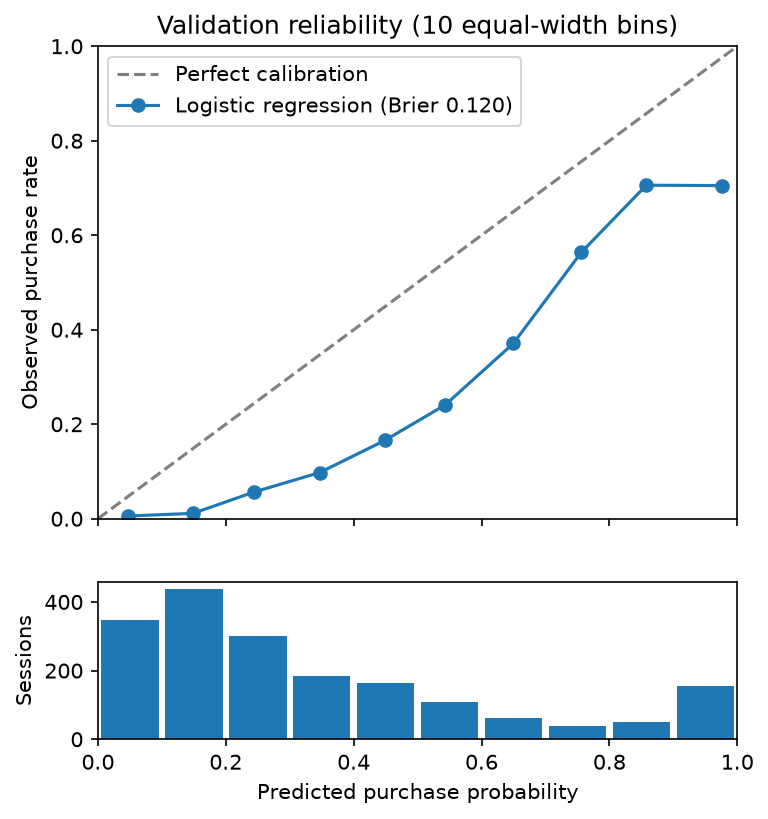
\includegraphics[width=0.6\columnwidth]{figures/reliability.png}
  \caption{\label{fig:reliability}
    Validation reliability plot for the selected model. Points below the
    dashed line are overestimates. The lower panel counts sessions per bin.}
\end{figure}

\paragraph{Class weighting and probability quality.} Table~\ref{tab:cv}
compares all eight settings. They fall within 0.013 AP of each other, well
inside the fold-to-fold standard deviation of about 0.028, so weighting and
the choice of $C$ make no clear difference to ranking. Weighting does clearly
hurt probability quality, raising mean Brier from about 0.085 to about 0.12.
On validation, the selected model's Brier score is 0.1197, only modestly
better than the class-prior baseline's 0.1308. The reliability plot
(Figure~\ref{fig:reliability}) shows that the model overestimates purchase
probability in every bin. For example, sessions in the 0.6--0.7 bin have an
average predicted probability of 0.65 but purchase only 37\% of the time.
The model ranks sessions usefully, but its probabilities should not yet be
read as purchase chances.

\section{Feedback and Plans}

During our consultation, we walked the TA through our preprocessing,
five-fold cross-validation setup and logistic regression results, and raised
our concern about class imbalance.

The TA suggested that a random baseline can be a useful comparison in some
cases, with performance above that baseline providing an initial check that
the model is learning useful information. We currently compare against
majority-class and class-prior baselines. The class-prior baseline gives
every session the same score, so it does not make random guesses. To follow
up on the advice, we plan to add a baseline that randomly predicts purchase
according to the training purchase rate and repeat it with several seeds
to show how much its results vary.

The TA also encouraged us to try models beyond logistic regression. We
explained that random forest and XGBoost are already part of our plan and
will be implemented next. Both can learn nonlinear relationships between
the session inputs. We will compare them using the same splits, training
folds and metrics, so any improvement can be assessed consistently.

\paragraph{What we will change.} Our first model changed the plan in two
ways. First, better ranking did not mean better probabilities. Class
weighting gave no clear AP gain but worse Brier scores, so we will treat
unweighted models as the default and compare them with models calibrated on
out-of-fold training predictions. We will not present the current weighted
probabilities as purchase chances. Second, the numeric inputs are heavily
skewed but enter logistic regression unchanged. We will test a
zero-preserving log transform within the training folds, while tree models
keep the original values. We also still need to run the feature-set study
with and without PageValues, and to inspect errors by month and visitor type.

\paragraph{Timeline.} We plan to finish random forest, XGBoost, tuning, the
feature-set study, calibration and error analysis by November 28. By
December 3, we will freeze the selected model and threshold, run the single
test evaluation and connect the saved pipeline to the Streamlit
demonstration. The final week is reserved for the report and demo.

\section*{Team Contributions}

Ankur worked on the project setup, dataset checks and exploratory
analysis. He also prepared the data splits and preprocessing pipeline used
for the model experiments.

\medskip\noindent Allen implemented the baseline models and logistic regression. He
evaluated their performance and prepared the results and figures used to
compare the models.

\medskip\noindent Krish organized the progress report and wrote the introduction and
related work. He also prepared the dataset and feature descriptions,
explaining the data properties and how the inputs are represented.

\section*{Generative AI Disclosure}

We used generative AI throughout this project, following the course policy.
As a team, we first discussed the overall goals and divided the work into
smaller tasks. We then used AI to turn the notes from those discussions into
the written GitHub issues we used to track the work. The decisions in that
plan, including the dataset, the models to compare and the evaluation
protocol, came from our own discussions.

Within individual tasks, we used AI for background research, for building
intuition about the methods we applied, and for writing parts of the code,
especially where we did not know the syntax of a library. We asked it to
explain the code it produced, so we could understand each step and remove
anything the task did not need, and we checked the results with our unit
tests and by rerunning the pipeline. We also used AI to help draft and edit
the text of this report. All reported numbers come from our saved result
files. We reviewed the AI-generated code and text and take full
responsibility for this submission.

\paragraph{Carbon footprint.} We did not record compute time, hardware or
region, so we used the course's estimate of 4.32\,g of CO$_2$ per query.
Across roughly 35 to 40 queries, this gives about 151 to 173\,g of CO$_2$.

% Bibliography entries for the entire Anthology, followed by custom entries
%\bibliography{custom,anthology-overleaf-1,anthology-overleaf-2}

% Custom bibliography entries only
\bibliography{custom}

% \appendix

% \section{Example Appendix}
% \label{sec:appendix}

% This is an appendix.

\end{document}
